\chapter{Title of chapter 2}

\section{Figures}

Figures are included as follows

\begin{figure}[h!] %the option h! forces the figure in this position
    \centering
    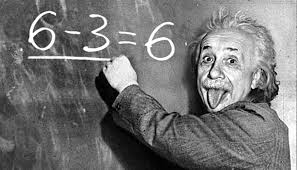
\includegraphics{example_figure.jpeg}
    \caption{Write the caption here}
    \label{fig:example_figure}
\end{figure}

and referred to in the text like this: Figure \ref{fig:example_figure}.
Put all your figures in the ``Figures'' folder.

\section{Tables}

Tables are constructed as follows

\begin{table}[t]
\caption{Write the caption here}. 
\label{tab:example_table}
\begin{tabu} to\linewidth{ X[2,l] | X[1,l] X[1,c] X[1,r] }
    \toprule 
    Column 1 has double space & Column 2 is left aligned & Column 3 is centred & Column 4 is right aligned \\
    \midrule 
    Value & Value & Value & Value \\
    \hline
    Value & Value & Value & Value \\
    \hline
    Value & Value & Value & Value \\
    \hline
    Value & \multicolumn3{l}{Like this you write on multiple columns}\\
    \hline
    Value & \multicolumn3{r}{also changing alignment}\\
    \bottomrule
\end{tabu}
\end{table}

and referred to in the text like this: Table \ref{tab:example_table}